% senior_thesis-proposal.tex
% Braden D. Licastro
% CMPSC 580, Spring 2013
%
% Oct 4, 2013
%
% This document provides a sample senior thesis proposal template for use
% by students in Allegheny's CS and Applied Computing programs.
%
%   *******************************************************************
%   * LOOK FOR BLOCK COMMENTS SUCH AS THIS ONE FOR AN EXPLANATION OF  *
%   * THIS DOCUMENT AND HOW TO MODIFY IT FOR YOUR OWN PROPOSAL!       *
%   *                                                                 *
%   * ANY LINE BEGINNING WITH A "%" IS A LATEX COMMENT AND IS IGNORED *
%   * BY THE LATEX PROCESSOR. YOU ARE ENCOURAGED TO COMMENT YOUR OWN  *
%   * LATEX CODE.                                                     *
%   *******************************************************************

%   ********************************************************************
%   * THE FIRST SECTION OF THE LATEX FILE IS THE "PREAMBLE." IT        *
%   * INSTRUCTS LATEX TO IMPORT SPECIAL PACKAGES FOR THINGS LIKE       *
%   * INCLUDING FIGURES, DOUBLE-SPACING, COLORED TEXT, ETC.            *
%   * DEPENDING ON YOUR NEEDS, YOU MAY FIND IT NECESSARY TO USE PACK-  *
%   * AGES THAT ARE NOT INCLUDED IN THIS TEMPLATE. SIMPLY IMITATE THE  *
%   * "\usepackage{...}" COMMANDS SHOWN BELOW.                         *
%   ********************************************************************

%   ********************************************************************
%   * BEGINNING OF PREAMBLE:                                           *
%   ********************************************************************
\documentclass[11pt]{article}

\usepackage[T1]{fontenc}
\usepackage{mathptmx}
\topmargin 0.0in
\setlength{\textwidth} {420pt}
\setlength{\textheight} {620pt} 
\setlength{\oddsidemargin} {20pt}
\setlength{\marginparwidth} {72in}
\setlength{\headheight}{14pt}

%   ********************************************************************
%   * Many of the commands below were simply copied over from an older *
%   * version of the proposal template; you can just leave them as     *
%   * they are (or you can delve into the TeX/LaTeX documentation      *
%   * and figure out what they do). Otherwise, jump ahead to the next  *
%   * block of comments, where you will enter title, abstract, etc.    *
%   ********************************************************************

\usepackage{fancyhdr} 
\usepackage[hyphens]{url}
\usepackage{graphicx}
\usepackage{epstopdf}
\epstopdfsetup{update} % only regenerate pdf files when eps file is newer

% set it so that subsubsections have numbers and they
% are displayed in the TOC (maybe hard to read, might want to disable)

\setcounter{secnumdepth}{3}
\setcounter{tocdepth}{3}

% define widow protection

\def\widow#1{\vskip #1\vbadness10000\penalty-200\vskip-#1}

\clubpenalty=10000  % Don't allow orphans
\widowpenalty=10000 % Don't allow widows

% this should give me the ability to use some math symbols that 
% were available by default in standard latex (i.e. \Box)

\usepackage{latexsym}

% define a little section heading that doesn't go with any number

\def\littlesection#1{
\widow{2cm}
\vskip 0.5cm
\noindent{\bf #1}
\vskip 0.0001cm 
}

\pagestyle{fancyplain}

\newcommand{\tstamp}{\today}   
\renewcommand{\sectionmark}[1]{\markright{#1}}
\lhead[\Section \thesection]            {\fancyplain{}{\rightmark}}
\chead[\fancyplain{}{}]                 {\fancyplain{}{}}
\rhead[\fancyplain{}{\rightmark}]       {\fancyplain{}{\thepage}}
\cfoot[\fancyplain{\thepage}{}]         {\fancyplain{\thepage}{}}

\newlength{\myVSpace}% the height of the box
\setlength{\myVSpace}{1ex}% the default, 
\newcommand\xstrut{\raisebox{-.5\myVSpace}% symmetric behaviour, 
  {\rule{0pt}{\myVSpace}}%
}

% leave things with no spacing extra spacing in the final version of the paper
\renewcommand{\baselinestretch}{1.0}    % must go before the begin of doc

% suppress the use of indentation for a paragraph

\setlength{\parindent}{0.0in}
\setlength{\parskip}{0.1in}

\begin{document}


% handle widows appropriately
\def\widow#1{\vskip #1\vbadness10000\penalty-200\vskip-#1}

% build the title section

\makeatletter

\def\maketitle{%
  %\null
  \thispagestyle{empty}%
  %\vfill
  \begin{center}%\leavevmode
    %\normalfont
    {\Huge \@title\par}%
    %\hrulefill\par
    {\normalsize \@author\par}%
    \vskip .4in
%    {\Large \@date\par}%
  \end{center}%
  %\vfill
  %\null
  %\cleardoublepage

  }

\makeatother

%   ********************************************************************
%   * Here is the first place where you need to begin customizing:     *
%   * Enter you name, the title of your proposal, etc., in the places  *
%   * indicated by the comment "% CHANGE!".                            *
%   ********************************************************************

\vspace*{-1.1in}
\title{Approximate Algorithmic Image Matching to Reduce Online Storage Overhead of User Submitted Images}  % CHANGE!

% build the author section
\author{
        Braden D. Licastro\\  % CHANGE!
        Department of Computer Science\\
        Allegheny College \\
        {\tt licastb@allegheny.edu}  \\  % CHANGE!
        \url{http://skynetgds.no-ip.biz/srthesis} \\   % CHANGE!
        \vspace*{.1in} \today \\ \vspace*{.1in}
}

\maketitle       % use the default title stuff

% Default "abstract" environment is too small; customize one instead:
\begin{center}
\large\bf Abstract
\vspace{-1em}  % Reduce space between header and the abstract
\end{center}

%   ********************************************************************
%   * Here is the second place where you need to customize:            *
%   * enter your abstract in the "quote" environment:                 *
%   ********************************************************************

\begin{quote}
Websites similar to Photobucket and imgur must be able to store massively increasing quantities of data. Most of these sites already implement systems that limit the number, size, and type of image, and compress the uploaded images to save space. Although these systems can be paired with file expiration times after which an upload is deleted, the cost of storage and backups of this data can be high. To address this problem, the research aims to create an intelligent image uploading system capable of identifying near-duplicate image uploads on-the-fly. This system also provide users with a higher resolution copy of their images from the server if available, thus providing better user experience while reducing unnecessary redundancy. By using the proposed system, users will benefit from improved quality and service while the business can reduce storage and other various costs.
\end{quote}

%\vspace*{-.4in}
\section{Introduction}
\label{sec:introduction}
\vspace*{-.1in}

%   ********************************************************************
%   * Enter the text of your introductory section here.                *
%   ********************************************************************

Computers are absolutely everywhere, and society is becoming more digitized every day creating
a need for storage of large amounts of data. When running a website, webmasters must manage storage space utilization, and the physical disks in the servers being used may not be centralized under one roof, 
but may in fact be located around the world. By allowing user submitted data, it quickly becomes 
apparent that data redundancy reduction can save a significant amount of storage space, especially 
when the data in question is backed up regularly. This research will target
the problem of data redundancy and provide a solution that will reduce not only storage costs but
also inefficiencies. An implementation of a duplicate-reducing image sharing website will be introduced that is
capable of managing large volumes of images using a database of identifiers and keys
that identify each individual file. By using this system, it is possible for the files to be stored in one
central location or distributed across several systems while avoiding excessive processing and wait times.
By using text based entries in a database, a hashing and collision resolution function can be 
implemented which is capable of producing a unique identification key for each file in the collection. 
Because this key is unique for each different file, it is a reliable gauge of uniqueness. 
When multiple files are found to be identical only one physical copy will be kept but 
multiple pointers to the database entry will allow easy access to the image from multiple locations.
On large, distributed network storage servers, the benefits become ever more apparent. As users upload images, the system will create an identifier for each file and search for a match in a database,
thus allowing the user to add to and access the data, but eliminate the overhead of storing numerous
copies of identical data. An increase in computation time will exist but should be minimal as
text comparisons will be the primary task in determining uniqueness, but this will be outweighed by
minimized physical storage requirements and costs of data backup.
The implementation of this system could be used in tandem with other methods of disk space cost reduction technologies. By not only using the proposed
method of duplicate reduction, it could in theory be possible that with image expiration times, file size maximums, and similar technologies, storage needs will plateau after the
initial surge of additions and the expiration time has passed for the earliest uploaded file. This
would allow webmasters to better predict overall needs and better predict upload trends and react
accordingly with preventative maintenance and any required space additions.

\vspace*{-.1in}
\section{Related Work}
\label{sec:relatedwork}
\vspace*{-.1in}

%   ********************************************************************
%   * Enter the text of your related work section here.                *
%   ********************************************************************

Though I will not be comparing existing images located in a database, the paper by Lee, Ke, and Isard \cite{Lee:2010} can be useful in method of approach. During their research they utilized a partition min-hash function for discovering near-duplicate images. Partition by hash functions are used to break down a large data set into a number of equal sized segments that can be identified by a generated hash. Instead of looking at the image as a whole as many other algorithms do, it looks at the image as several smaller pieces through the use of the partition hashing function. They claimed that the algorithm is actually faster and more effective than standard min-hash functions which look at the entire image. Since the proposed research I will be performing is highly efficiency sensitive due to its web based structure, I will consider implementing a variant of this method of comparison.

Another article that will be vital to creating an effective and efficient image matching algorithm will be the 2010 paper by Srinivasan. This research was targeted at web-based image matching, which is exactly what I am going to perform. This research claims that traditional near-duplicate detection systems are not applicable for the de-duplication of large-scale web image collections, \cite{Srinivasan:2008} the research performed targeted an image matching system which was scalable, highly efficient, and effective.

In order to perform the effective image matching the authors required, they decided to implement a thumbnail matching based system. This algorithm would generate a 130-bit thumbnail representation of the image and was capable of finding near-duplicate images while operating in $O(1)$ time \cite{Srinivasan:2008}.

\begin{figure}[htbp]
\centering
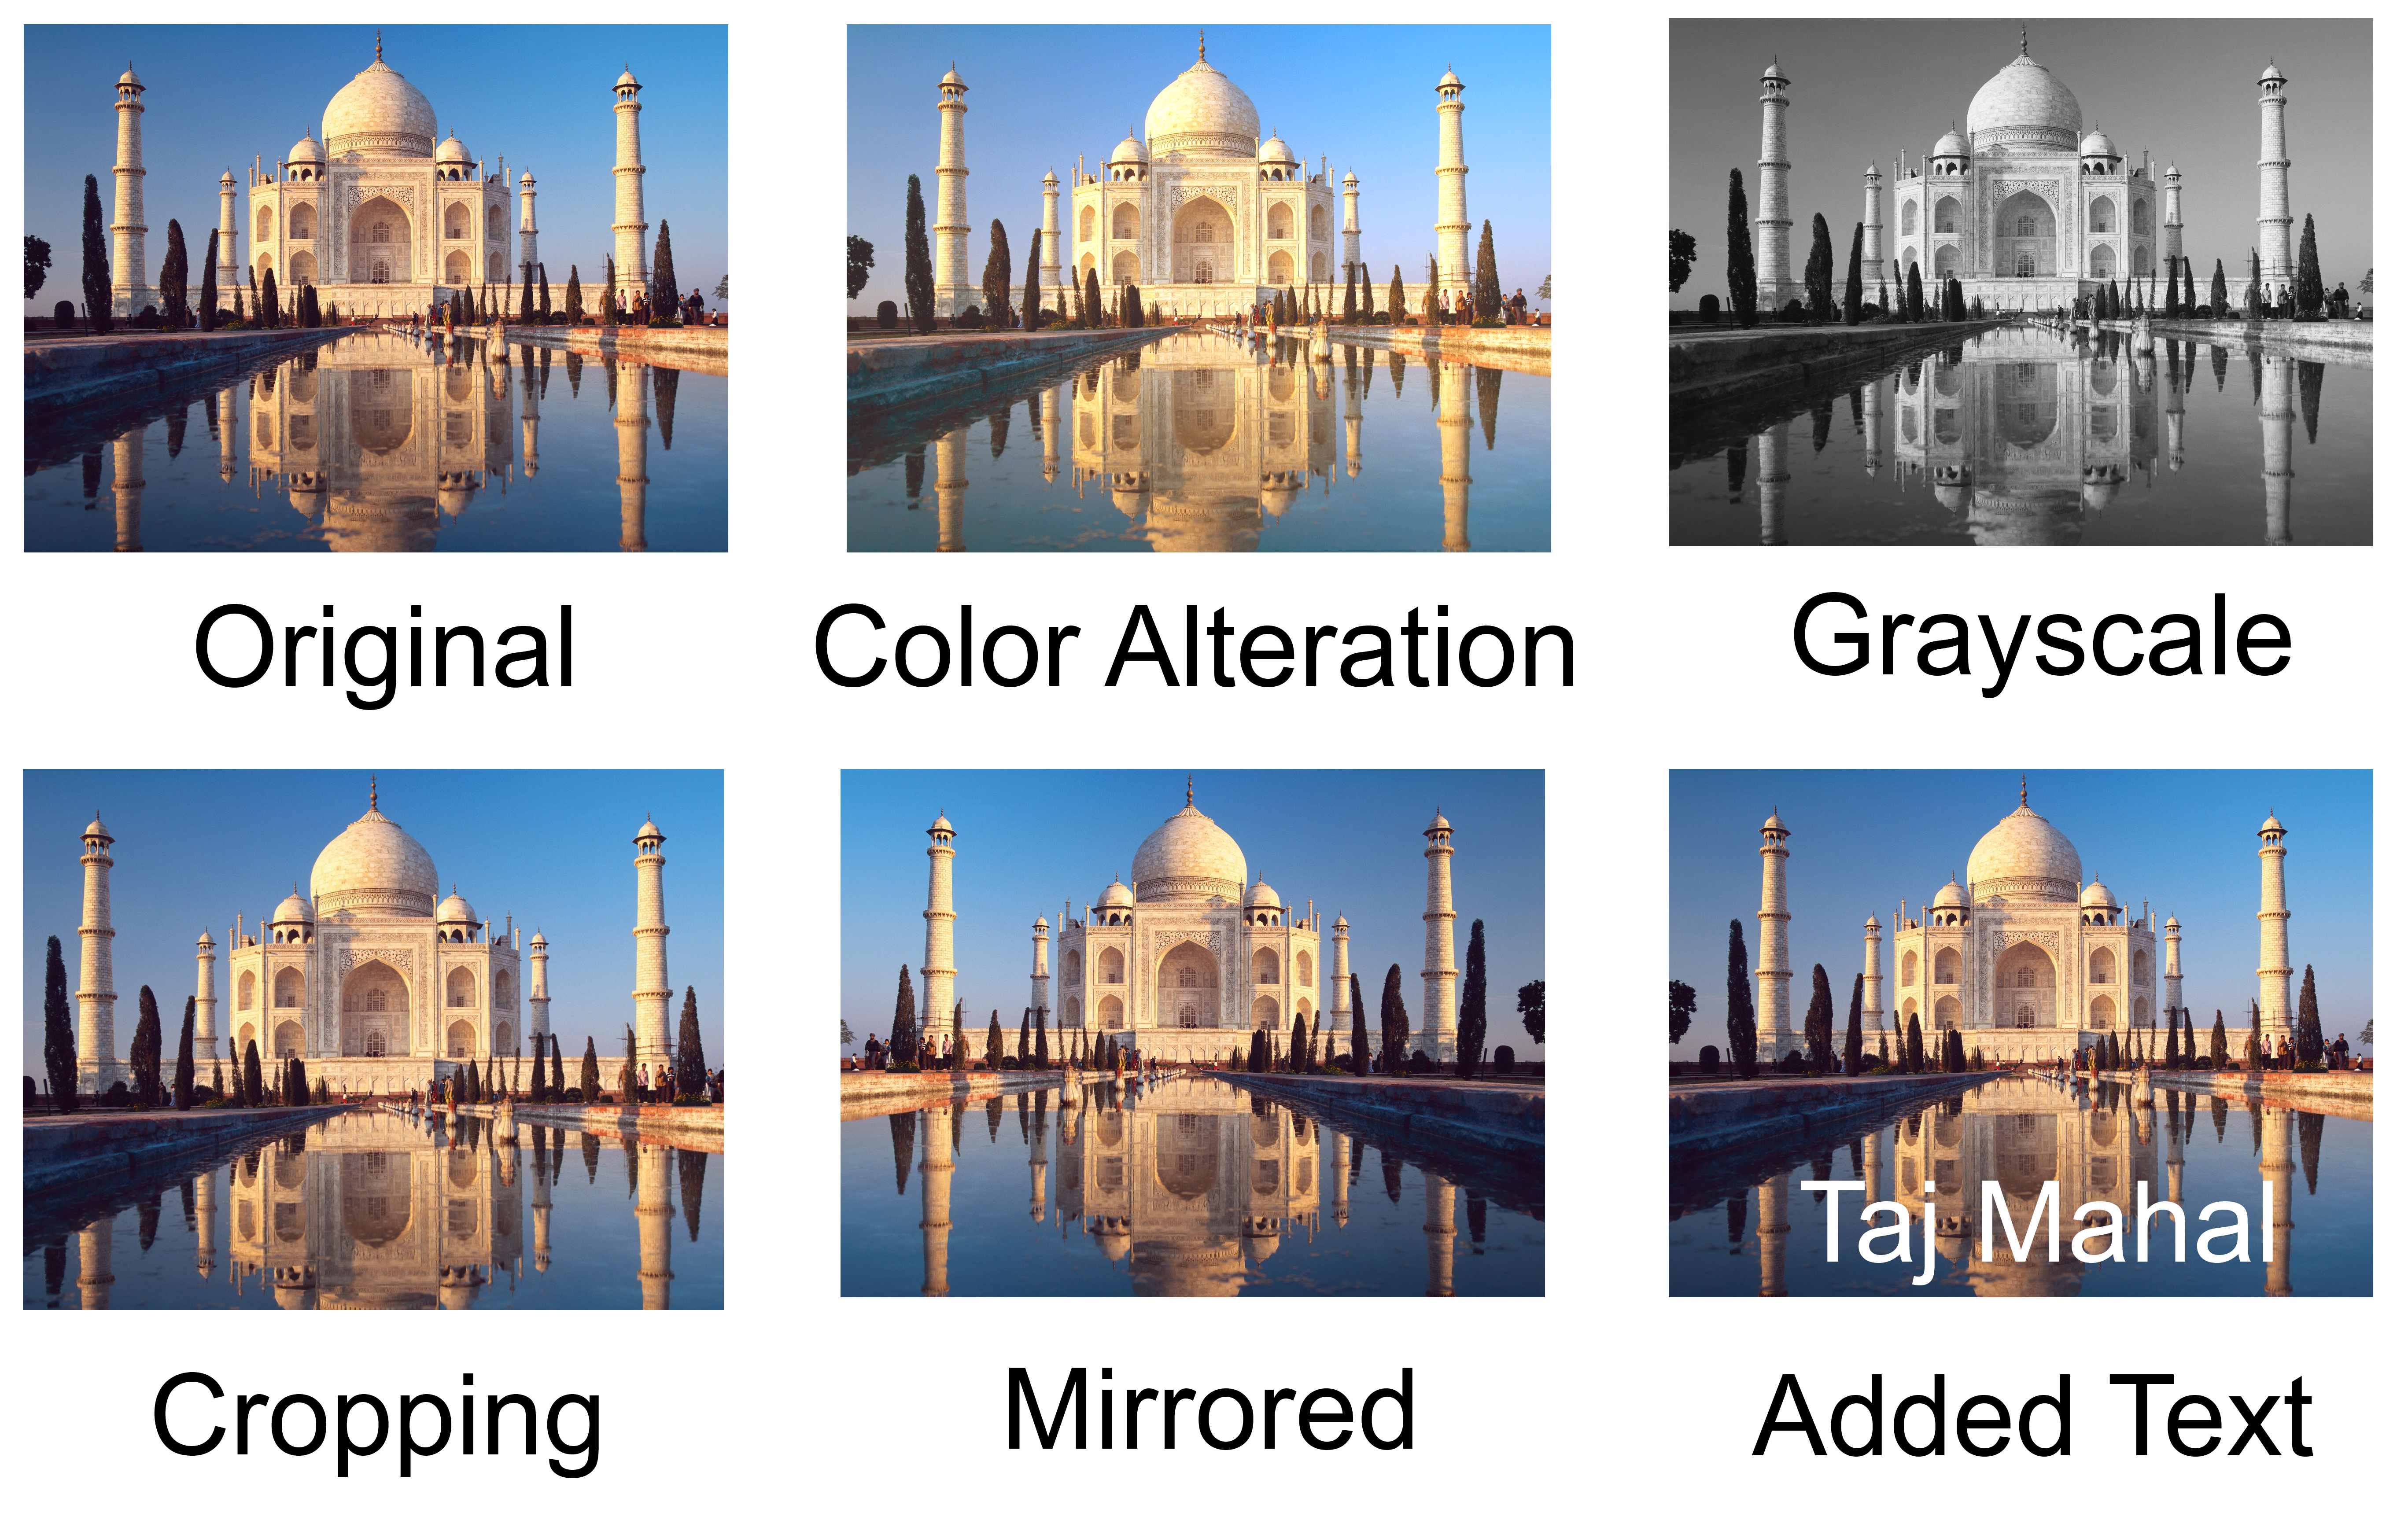
\includegraphics[width=3.5in]{imagesamples}
\caption{Possible image manipulations}
\label{imgsample}
\end{figure}

When using this thumbnail method, the authors were able to adjust automatically for differences in resolution, arbitrary amounts of cropping, caption, logo, and other manipulations, in addition to color and rotation variations, examples which can be seen in figure \ref{imgsample}. Implementing this method could benefit the research being proposed, as each of these are highly probable manipulations, and will likely each be included in the final tests performed on the implemented system.

Due to the web based nature of the proposed research, another article, written by Foo, Zobel, Sinha, and Tahaghoghi in 2007 focuses primarily on web search based image matching \cite{Foo:2007}. Their research primarily targets the finding and determination of types of copyright infringement as most near-duplicate images are derived from one source. The goal of their research was not to derive an algorithm capable of matching images, but to locate duplicate and near-duplicate images on the web using search engines, and determine the most common methods of image alteration leading to redundancy and possibly copyright infringement. Their research will be invaluable to the proposed research as it will then be possible to target the most common methods of image alteration when creating a matching algorithm. To locate their image set to work with, they used the most popular search queries of 2005 and collected the number of images, and determined the number of unique images based on the results returned. As a note, images with non-unique URLs were not included to prevent false duplicates from the same sites. In conclusion, the authors found that the most common alterations, ordered from one to 10, one being the most common, were as follows \cite{Foo:2007}:
\begin{enumerate}
\item
\textbf{Combination:} Images with more than one alteration.
\item
\textbf{Scale:} Images that differ in size.
\item
\textbf{Crop/Zoom:} Images that are cropped from the original.
\item
\textbf{Picture in Picture:} Images that contain another image.
\item
\textbf{Contrast:} Images that have adjusted contrast.
\item
\textbf{Border/Frame:} Images that have added borders or frames.
\item
\textbf{Grayscale:} Images that have been converted to grayscale.
\item
\textbf{Recoloring:} Images with colors that have been modified.
\item
\textbf{Mirror:} Images that have been mirrored to prevent copyright infringement detection.
\item
\textbf{Rotate:} Images that have been rotated.
\end{enumerate}

The research proposed will not focus on every one of these common parameters that have been found, but will focus on a select group of these common alterations outlined in section \ref{sec:evaluate}.

Finally, the most relevant information found will provide a starting codebase for the algorithm and research. An online coding tutorial provider, CatPa, outlined a method of using PHP libraries to generate real-time thumbnails and hashes of images and compare them to ones currently located on a server before uploading \cite{catpa:gdcode}. If the image is a duplicate it would be denied the privilege of being uploaded and the function would notify the user. This system is extremely limited as it provides the user with no way of adding an image to the server if it is not a duplicate and is only a false positive, and if it is unique, does not provide them with a method of accessing the already-present file.

The image comparison code developed by CatPa will be used as a base to generate a fully functional image sharing site with duplicate-reduction systems and allow for the testing of the effectiveness of such a system over traditional methods of sharing with duplicates allowed. The system created by the author\cite{catpa:gdcode} generates a $16\times 16$ thumbnail of each image on the server, and of the image being uploaded. From here, the algorithm will generate and compare black and white and color histograms, the thumbnails, and determine if it is a duplicate based on the allowable difference threshold setting which will be determined after running initial tests outlined in section \ref{sec:evaluate} and analyzing the results \cite{catpa:gdcode}. The proposed research will utilize this exact method, but will provide code improvements to utilize less memory by implementing the PHP Improved libraries and also checking images for immediate similarities in resolution, exact image matching with a full MD5 image hash, and by comparison of metadata. These methods require minimal calculation, just a simple comparison of strings compared to the generation of histograms and resizing of images. After the initial string comparison approach, the code will be used to calculate the average deviation between the two images and will allow easy expansion of the system to provide a faster, more effective image matching system.

\vspace*{-.2in}
\section{Method of Approach}
\label{sec:method}
\vspace*{-.1in}

%   ********************************************************************
%   * Enter the text of your method of approach section here.          *
%   ********************************************************************
In order to implement the proposed research, the website will be run on a custom server with an allocated 5 gigabytes of dedicated storage, 8 gigabytes of RAM, and a Core i3 2.43 GHz processor. All services and programs will be shut down during the experiment except for Apache, MySQL, PHP, and Webmin to ensure consistent results. Throughout the duration of the experiment, no software updates will be installed other than security related operating system updates. The website must be designed to be lightweight, have no extraneous scripts or applets running on the upload page, and will be compatible with WebKit browsers such as Firefox. This limitation will allow for a focused effort in file management on a specific platform and will allow room for further research after the tool has been optimized. To start, a database will be implemented so that it is able to hold a hashed key for each uploaded image and the location of the file on the disk in addition to upload statistics to complete the task. An example of this schema can be seen in figure \ref{fig:schema}.

\begin{figure}[htbp]
\centering
\includegraphics[width=5in]{schema}
\caption{Proposed schema for file uploads}
\label{fig:schema}
\end{figure}

The website will run multiple scripts for each upload. The first script will be a traditional upload method where the user supplies a file, it will be uploaded to the server, and the server will return a unique URL from which to access the image at a later time. During this process, each file will be assigned a new, unique name to prevent collisions upon upload. A SQL {\tt "INSERT"} will then be run on the database for the image and will record the file's location on the server, the file name, the fact it was uploaded using the traditional method, the unique URL to access it from, and an {\tt ID} for each insert into the database. After the completion of the process an {\tt "UPDATE"} will be run on the database entry created by the {\tt "INSERT"} above. The time taken to complete the task will be included in that entry and can be used to analyze the efficiency of both systems upon the completion of the tests outlined in section \ref{sec:evaluate}.

After the first script completes, a second script will be called. This will perform mostly the same function as the traditional upload script, but will check the image being uploaded for duplicates and handle each case appropriately. The image will be taken and converted into a $16\times 16$ black-and-white thumbnail and a histogram will be produced from that image. The server will then look into the database and check whether or not any images uploaded with the duplicate reduced system are similar to the one looking to be uploaded. If there are no matches, then the image upload will be accepted by the function and stored on the servers disk. At this time a SQL {\tt "INSERT"} will then be run on the database for the image and will record the files location on the server, the file name, the fact that it was uploaded using the duplicate-reduced method, the unique URL to access it from, the image's MD5 hashed histogram that is described below, and an {\tt ID} for each insert into the database. After the completion of the process an {\tt "UPDATE"} will be run on the database entry created by the {\tt "INSERT"} above.

If the image histogram hash matches the hash on the server, a color profile will be generated in real time for both images and compared pixel by pixel. If there is a match or close match, the script will compare several small, randomly chosen blocks on the images. If these match, then the image is assumed to be a duplicate and a prompt will be displayed to the user showing them the image they provided and the possible match that already exists. If the image is verified a match, the higher of the two resolutions will be kept, and the user will be given a unique link to the image. If the user decides the image is not a duplicate, the system will run an {\tt "INSERT"} on the database as outlined earlier, and it will be added to the database. Following the completion of this process an {\tt "UPDATE"} will be run on the last {\tt "INSERT"} and the time taken to complete the task will be included in that entry.

In the case of requiring duplicate files, where the user decides to upload the image regardless of uniqueness, the script will be able to differentiate between the two images with the unique image ID that is generated at the time of insertion into the database. The closest matching occurrence of an image on the server compared to a new upload will be used in the prompt displayed to the user. This will prevent frustration with multiple prompts every time more than one duplicate is found.

If an image is indeed found to be duplicate, and the user chooses to use the higher resolution image that is on the server, a unique link will be generated, displayed to the user, and an {\tt "INSERT"} statement will be run containing the same information as the matching file's insert did at the time of upload. This will allow multiple links that point to the same image and the user will be unaware of the system operating in the background which will provide a consistent experience. An outline of this full process can be seen in figure \ref{method-fig1}.

\begin{figure}[htbp]
\centering
\includegraphics[width=5in]{upprocess}
\caption{Streamlined upload process}
\label{method-fig1}
\end{figure}

When a user accesses the file from the provided link, the system will run a query that looks up the image identifier provided in the URL. If it matches an image on the server, the image location will be used to provide the image to the user for viewing. The user never notices a difference, but on the server side we have ensured file redundancy has been eliminated and possibly improved user experience by providing the user with higher quality content than what they were expecting. If the image is not found, a 404 "Image cannot be found." error will be displayed to let the user know something went wrong.

%Left the figures intact temporarily for future reference in case I need a table.
%
%\begin{figure}[htbp]
%\centering
%\includegraphics[width=5in]{flow}
%\caption{Flow graph for proposal-writing}
%\label{intro-fig1}
%\end{figure}
%
%\begin{table}[htbp]
%\centering
%\begin{tabular}{|c||c|c|}
%\hline
%\bf Task & \bf Begin Date & \bf End Date\\\hline\hline
%First draft & Now & 20 Sept\\\hline
%Second draft & 20 Sept & 27 Sept\\\hline
%Third draft & 27 Sept & 4 Oct\\\hline
%Fourth draft & 4 Oct & 11 Oct\\\hline
%Fifth draft & 11 Oct & 18 Oct\\\hline
%\end{tabular}
%\caption{Proposed work schedule}
%\label{intro-tab1}
%\end{table}

\vspace*{-.2in}
\section{Evaluation Strategy}
\label{sec:evaluate}
\vspace*{-.1in}

%   ********************************************************************
%   * Enter the text of your evaluation strategy section here.         *
%   ********************************************************************

Evaluating the effectiveness of the website will entail several benchmark readings. The total number of files, number of unique files, and the overall size of the benchmark folder versus the duplicate reduced upload folder will all be used in determining the effectiveness of the image comparison algorithms implemented in the website. To perform the tests, a fixed set of standardized test images from TecNick will be used \cite{tecnick:testimage}. These images will consist of a collection of 15 artificially generated gray-scale, 15 natural gray-scale, and 15 natural RGB images in addition to 5 duplicate images in each category. A survey posted by NTP Software stated that approximately 20\% of data on storage systems can be attributed to duplicate data \cite{ntps:staledata}. By using 15 unique and 5 duplicate images in each category, it is possible to represent this average and determine how effective the reduction method is. The duplicates will consist of one of each of the following images: identical, diminished resolution, text overlaid, reduced size, and a color/contrast correction.

\begin{figure}[htbp]
\centering
\[\left ( \frac{Base - Reduced}{Base} \right ) * 100 = \% Improvement Over Base\]
\caption{Equation for determining efficiency improvements}
\label{benchmark_eq}
\end{figure}

In order to test the algorithm, all 15 unique images will be uploaded to the server using the built in upload function. Any false positive matches will be noted and the algorithm will be adjusted to reduce the number of false positives. At this point, the baseline folder and the duplicate reduced folders should contain the same set of data. Next, the duplicate images will be uploaded to the server using the same method. The system should find all remaining images as duplicates and prompt the user with the option to upload anyway or use the existing image. For the test I will not allow the upload. After all images have been uploaded, the total number of files in the baseline directory will be compared to the number of files in the duplicate reduced directory using the algorithm in figure \ref{benchmark_eq}, where base is the baseline directory number to be compared and reduced is the duplicate reduced directory number to be compared.  The directory sizes and average upload times will also be evaluated using the algorithm in figure \ref{benchmark_eq}. The evaluated result, if positive, will denote a positive improvement in efficiency compared to the baseline directory, and a negative result is interpreted as a decrease in efficiency over the baseline directory.

After analyzing the results of the test outlined above, the algorithm will be refined to provide more accurate results and the folders and database will be reset. At this point, the tests will be run again, and any changes in effectiveness will be noted. Because the system implements a text-based database, the size difference between the baseline and duplicate reduced will be negligible as no image specific information is stored. In addition, the number of entries will be identical due to the upload process outlined in \ref{sec:method}, which generates a unique URL for every image upload request whether the image is uploaded or an existing one on the server is used.

\vspace*{-.1in}
\section{Research Schedule}
\label{sec:schedule}
\vspace*{-.1in}

The research schedule for the project is to be tentatively based on the following deadlines.
Due to the nature of the project and the wide array of pre-existing software required needing to
be modified and implemented, unseen hurdles may arise.

Phase 1:1 month: Find acceptable operating system, set up a fully functional LAMP server to host website and provide storage of submitted images. During this time, I will begin learning and installing PHP and JavaScript libraries so code implementation can begin shortly after the completion of server setup.

Phase 2:2-3 months: Develop a working image sharing website which is capable of satisfying the requirements
outlined in \ref{sec:method}. Set up two basic file and database structures to be used throughout the experiment. One will be used as a baseline and the other structure will function as the duplicate-reduced system. Both will host the image files, file information, and time taken to add files to the database. The system will also track the average upload time for each method, the total number of files, and the total size of each upload directory.

Phase 3:1 week: During this time I will run various tests on the website using the proposed
methods in \ref{sec:method} and record the results of the experiment. After the new image files have been added to the collection, some unique, and others duplicate, the submissions directory on the server will be scanned for  duplicates and ensure none were accidentally added. Results to be recorded are the final number of files, the number of duplicate images, and the total storage space used.

Phase 4:Remaining time: The results gathered throughout the test process will be evaluated and
the website algorithms tweaked and finalized. After modifications are complete tests will be rerun and the
final results will be evaluated.
\vspace*{-.1in}
\section{Conclusion}
\label{sec:conclusion}
\vspace*{-.1in}

%   ********************************************************************
%   * Enter the text of your concluding section section here.          *
%   ********************************************************************

With computers becoming ever more prevalent and data being generated and shared at a rapidly increasing rate, it is becoming more and more necessary every day to reduce the redundancy of shared data and create more efficient sharing systems. By removing duplicate image files from
sharing sites and preventing the addition of new duplicates we can begin to tackle this issue and begin reducing the storage requirements of running such systems. Aside from just reducing storage overhead it can also be possible to reduce time overhead of searching for images and the amount of bandwidth needed to operate these systems. In addition, a significant amount of money can be saved as a result of reduced electrical costs per node, and even reduce the number of server nodes in extreme cases of redundancy.

\newpage
\nocite{*}
\bibliographystyle{plain}
\bibliography{senior_thesis_proposal}

\end{document}

